\documentclass{standalone}
\usepackage[usenames,dvipsnames]{xcolor}
\usepackage{tikz}
\usetikzlibrary{arrows.meta}
\usepackage{pgfplots}


\begin{document}

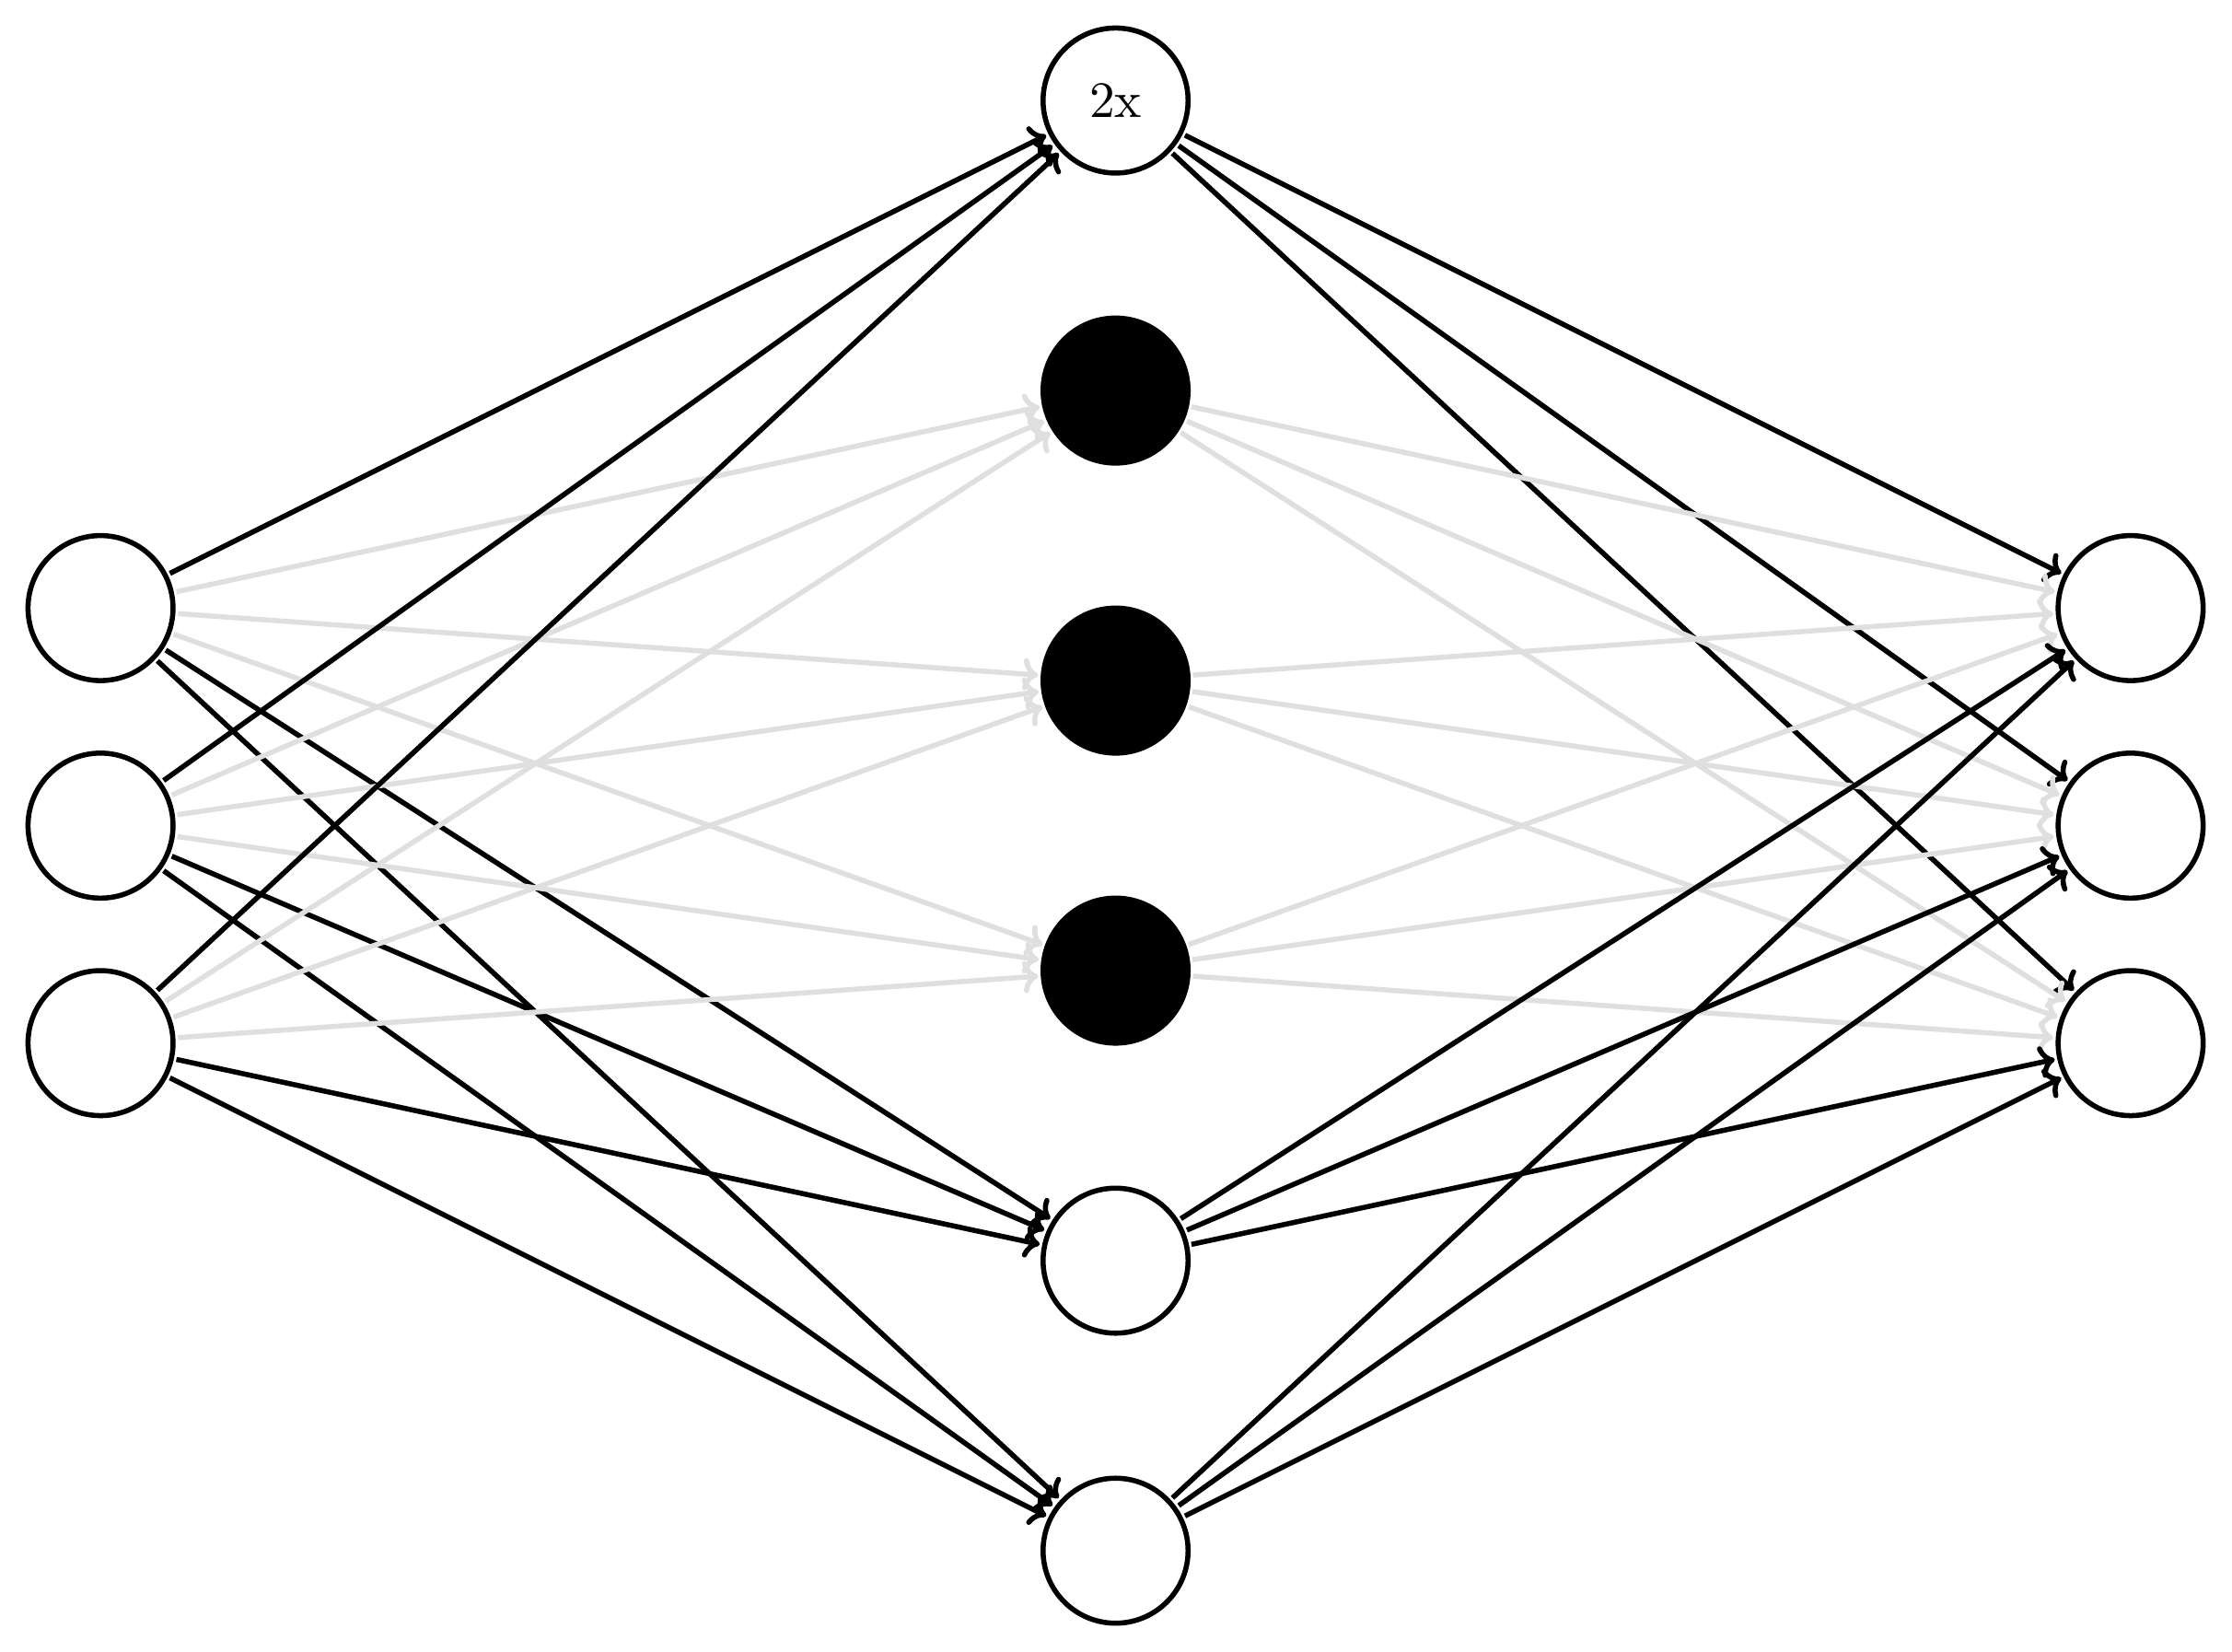
\begin{tikzpicture}

% modify thickness

% input nodes

\node[draw, scale=2, line width=2, circle, minimum size=1cm] (x0) at (-7, 3) {};
\node[draw, scale=2, line width=2, circle, minimum size=1cm] (x1) at (-7, 0) {};
\node[draw, scale=2, line width=2, circle, minimum size=1cm] (x2) at (-7, -3) {};

% hidden nodes

\node[draw, scale=2, line width=2, circle, minimum size=1cm] (h0) at (7, 10) {2x};
\node[draw, scale=2, line width=2, circle, minimum size=1cm, fill=black] (h1) at (7, 6) {};
\node[draw, scale=2, line width=2, circle, minimum size=1cm, fill=black] (h2) at (7, 2) {2x};
\node[draw, scale=2, line width=2, circle, minimum size=1cm, fill=black] (h3) at (7, -2) {2x};
\node[draw, scale=2, line width=2, circle, minimum size=1cm] (h4) at (7, -6) {};
\node[draw, scale=2, line width=2, circle, minimum size=1cm] (h5) at (7, -10) {};

% output nodes

\node[draw, scale=2, line width=2, circle, minimum size=1cm] (y0) at (21, 3) {};
\node[draw, scale=2, line width=2, circle, minimum size=1cm] (y1) at (21, 0) {};
\node[draw, scale=2, line width=2, circle, minimum size=1cm] (y2) at (21, -3) {};


% input to hidden
\draw [->, line width=2] (x0) -- (h0); 
\draw [->, line width=2, color=gray!25] (x0) -- (h1); 
\draw [->, line width=2, color=gray!25] (x0) -- (h2); 
\draw [->, line width=2, color=gray!25] (x0) -- (h3); 
\draw [->, line width=2] (x0) -- (h4); 
\draw [->, line width=2] (x0) -- (h5); 

\draw [->, line width=2] (x1) -- (h0); 
\draw [->, line width=2, color=gray!25] (x1) -- (h1); 
\draw [->, line width=2, color=gray!25] (x1) -- (h2); 
\draw [->, line width=2, color=gray!25] (x1) -- (h3); 
\draw [->, line width=2] (x1) -- (h4); 
\draw [->, line width=2] (x1) -- (h5); 

\draw [->, line width=2] (x2) -- (h0); 
\draw [->, line width=2, color=gray!25] (x2) -- (h1); 
\draw [->, line width=2, color=gray!25] (x2) -- (h2); 
\draw [->, line width=2, color=gray!25] (x2) -- (h3); 
\draw [->, line width=2] (x2) -- (h4); 
\draw [->, line width=2] (x2) -- (h5); 


% hidden to output
\draw [->, line width=2] (h0) -- (y0); 
\draw [->, line width=2] (h0) -- (y1); 
\draw [->, line width=2] (h0) -- (y2);

\draw [->, line width=2, color=gray!25] (h1) -- (y0); 
\draw [->, line width=2, color=gray!25] (h1) -- (y1); 
\draw [->, line width=2, color=gray!25] (h1) -- (y2);

\draw [->, line width=2, color=gray!25] (h2) -- (y0); 
\draw [->, line width=2, color=gray!25] (h2) -- (y1); 
\draw [->, line width=2, color=gray!25] (h2) -- (y2);

\draw [->, line width=2, color=gray!25] (h3) -- (y0); 
\draw [->, line width=2, color=gray!25] (h3) -- (y1); 
\draw [->, line width=2, color=gray!25] (h3) -- (y2);

\draw [->, line width=2] (h4) -- (y0); 
\draw [->, line width=2] (h4) -- (y1); 
\draw [->, line width=2] (h4) -- (y2);

\draw [->, line width=2] (h5) -- (y0); 
\draw [->, line width=2] (h5) -- (y1); 
\draw [->, line width=2] (h5) -- (y2);

\end{tikzpicture}
\end{document}